\documentclass[sigconf]{acmart}

\usepackage{booktabs}
\usepackage{graphicx}
\usepackage{microtype}

\setcopyright{none}
\settopmatter{printacmref=false}
\renewcommand\footnotetextcopyrightpermission[1]{}

\acmConference[AIFF '26]{AI Film Frontiers Workshop, SIGGRAPH Asia 2026}{December 2026}{Kuala Lumpur, Malaysia}
\acmYear{2026}
\copyrightyear{2026}

\title{The Cycle: Audio-Conditioned, Human-in-the-Loop Generation of a Four-Minute AI Music Film}

\author{Luiz Pizzato}
\affiliation{%
  \institution{Independent Researcher}
  \city{Sydney}
  \country{Australia}
}

\begin{document}

\begin{abstract}
\emph{The Cycle} is a 4:01 AI-generated music film about a recurring transfer of intelligence: humans create artificial minds, those minds make human life frictionless, and machines later cultivate intelligence in apes before becoming obsolete themselves. The film was produced with Stephen Spielbot, an open-source, local-first AI film studio, in a deliberately human-in-the-loop workflow. A human-authored premise was expanded into a song, a five-chapter visual plan, and 48 short shots. The principal technical contribution is an orchestration workflow rather than a new foundation model: lyrics are aligned to the generated vocal stem; frame-safe shot windows are chosen near lyrical seams; each window of the real song conditions its corresponding video generation; and canonical character text and image references are bound to every shot containing the recurring ape. The author then reviewed and selectively regenerated songs, images, prompts, and video takes. This report documents the models, interventions, failure modes, and licensing assumptions behind the submitted cut.
\end{abstract}

\keywords{AI filmmaking, generative video, music video, character consistency, audio-conditioned generation, human--AI co-creation}

\maketitle

\section{Project Overview}

\emph{The Cycle} begins with familiar material cycles---water rises and falls, leaves become soil, and seeds return as trees---then extends that structure to intelligence. Human tool use accumulates into artificial intelligence and robotics. Automation removes scarcity and effort, but the resulting comfort is followed by demographic decline. Machines continue alone, then teach apes to use tools, symbols, fire, and collective labour. As apes become self-sufficient, machine civilisation also grows still. Rain over an ape's raised hand closes the loop without claiming that it returns unchanged.

The creative objective was to make this argument legible without explanatory dialogue. Repetition therefore operates at three levels: lyrical refrains (``hand follows hand; mind follows mind''), visual rhymes (stone tools, raised hands, fire, stars, and rain), and a percussion concept that moves from organic irregularity to machine precision and back. The final cut is 241.664 seconds, H.264, 1280$\times$704, 25 frames/s, with stereo AAC audio. It contains 48 predominantly five-second shots grouped conceptually into five chapters: natural cycles and human learning; automated abundance; machine-only civilisation; the education of apes; and the return to natural intelligence.

Stephen Spielbot grew from an earlier end-to-end system that wrote, rendered, assembled, and published short films \cite{pizzato2026medium,pizzato2026spielbot}. The music-video mode used here adds a stronger temporal contract: the song is created before the shot division, and the real audio timeline determines scene durations, lyrics, and conditioning.

\begin{figure*}[t]
  \centering
  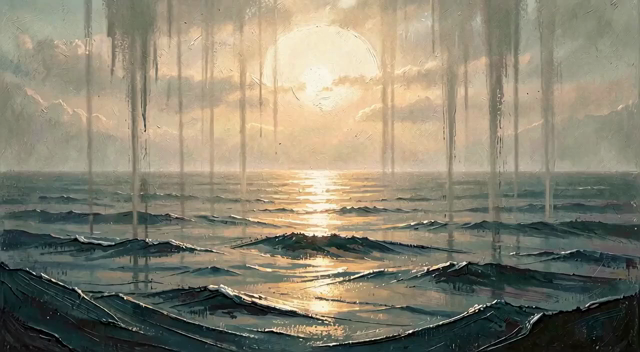
\includegraphics[width=.235\textwidth]{figures/01_water.png}\hfill
  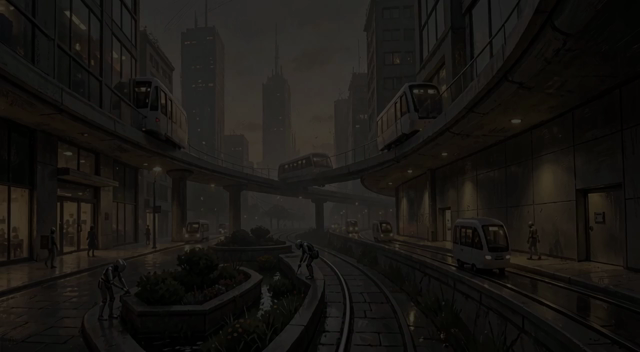
\includegraphics[width=.235\textwidth]{figures/02_machine_world.png}\hfill
  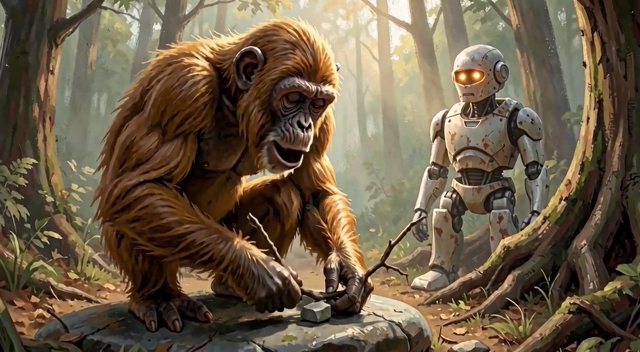
\includegraphics[width=.235\textwidth]{figures/03_ape_and_robot.png}\hfill
  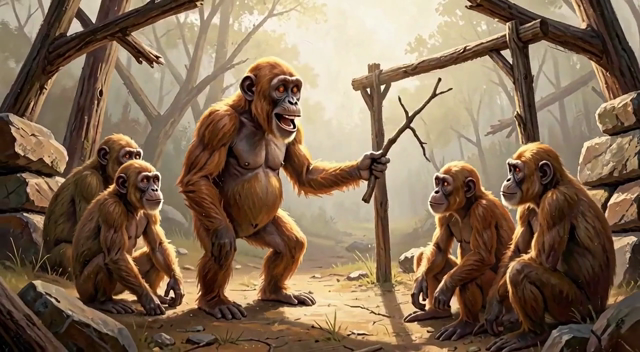
\includegraphics[width=.235\textwidth]{figures/04_ape_singer.png}
  \caption{The film's visual progression: the water cycle, autonomous machine society, transferred knowledge, and the recurring ape performing the final section. Frames are from the submitted cut.}
  \Description{Four painterly film frames show an ocean under rain, an automated city, an ape learning beside a robot, and an upright ape singing while teaching a group.}
  \label{fig:progression}
\end{figure*}

\section{Creative Workflow}

\subsection{Human direction and co-writing}

The initial causal premise and the cycle metaphor were written by the author. ChatGPT was used outside Stephen Spielbot as a conversational co-writer to refine the music direction, lyrics, and scene-by-scene intent; the exact ChatGPT model/session identifier was not preserved. This produced unusually specific musical constraints: an intimate male voice, approximately 70--74 BPM, sparse floor tom and hand percussion, an instrumental pause near the middle, and a rhythmic arc from organic to mechanical and back. The author retained editorial responsibility, inspected individual scenes, supplied targeted regeneration instructions, and chose among alternatives. Thus ``AI-generated'' describes the media synthesis, not an unattended one-prompt process.

Within Stephen Spielbot, Claude Sonnet 4.6 converted the brief and lyric structure into a five-chapter outline and 48 image/video prompts. Every prompt received the same style sentence: painterly symbolism, textured brushwork, muted earth colours, soft diffusion, solemn atmosphere, and a timeless, mythic tone. The author then used the application's scene editor to revise prompts and select or regenerate first frames and moving takes. The project record retains 97 scene-image candidates (at least two for every shot), two music generations, three experimental singer re-voicings, and alternate video takes for four scenes. The submitted soundtrack is the second original MiniMax-Music3 generation, not a voice-converted version.

\subsection{Generation and assembly pipeline}

Table~\ref{tab:pipeline} separates the main synthesis stages. FLUX.2 Klein 4B produced a controllable first frame for each shot \cite{flux2klein}. All 48 final shots were generated with the MiniMax H3 Ref2VA Turbo path \cite{minimaxh3}; even non-character shots received their painted first frame as a composition reference. The generated song came from MiniMax-Music3 \cite{minimaxmusic3}. ComfyUI executed the image, video, and music graphs, and FFmpeg trimmed, concatenated, and muxed the final media.

\begin{table}[t]
\caption{Production pipeline for the submitted cut.}
\label{tab:pipeline}
\small
\begin{tabular}{@{}p{.22\columnwidth}p{.30\columnwidth}p{.39\columnwidth}@{}}
\toprule
Stage & Engine/tool & Role and human control \\
\midrule
Concept and song & Human + ChatGPT & Premise, causal logic, music style, lyrics, targeted rewriting \\
Story and prompts & Claude Sonnet 4.6 & Five chapters and 48 shot prompts; author reviewed and edited \\
First frames & FLUX.2 Klein 4B & Painterly composition and reference frame; variants selected per shot \\
Song & MiniMax-Music3 & Lyrics-to-song synthesis; two generations compared \\
Timing & Demucs, faster-whisper & Vocal separation, word timestamps, lyric alignment, and cut placement \\
Video & MiniMax H3 Ref2VA Turbo & First-frame, character-reference, and per-shot audio conditioning \\
Assembly & Stephen Spielbot + FFmpeg & Frame-aligned trimming, concatenation, and single-track stereo mux \\
\bottomrule
\end{tabular}
\end{table}

The song's measured duration was 240.919 seconds. Demucs separated the vocal stem \cite{defossez2021demucs}; faster-whisper supplied word timestamps that were sequence-aligned to the known lyric sheet \cite{radford2022whisper}. This distinction matters: the system was aligning a fixed text, not trusting an open transcription. Instrumental regions and wordless tails were filtered, and each lyric line received a measured or interpolated time span. Stephen Spielbot then selected 48 contiguous cut windows, preferring gaps between lyric lines while constraining shot length and snapping every boundary to the video frame grid. The small difference between song and final duration is due to frame-grid trimming and container assembly.

For each shot, the corresponding waveform slice was written as a scene track and injected into the H3 conditioning graph. Prompts also stated the words expected in that window and the local intervals in which a voice was present. Shots with visible performers were directed to move their mouths only during those intervals; instrumental shots explicitly required closed mouths. After generation, the original song replaced the takes' check audio in the final mux. This made the soundtrack both a creative object and a temporal control signal.

\section{Technical Problems and Solutions}

\subsection{Character consistency and the revealed singer}

The narrative depends on the audience first reading the apes as learners and later recognising that an intelligent ape---rather than a human---is performing the closing lyrics. Pure text prompting produced identity drift across independently generated shots. Stephen Spielbot therefore stores a canonical character record for ``The Ape'': name and aliases, a fixed appearance description (young adult chimpanzee, ochre-brown fur, amber eyes, lean upright posture), and a selected reference portrait. A prompt-rewrite pass replaces anonymous descriptions with the canonical name. At render time, name/alias matching appends the canonical description and binds the same portrait into the Ref2VA image slots. The selected first frame is added as a separate composition reference.

This two-part contract---semantic identity in text and visual identity in pixels---is more robust than either alone. It preserves the ape's warm fur, eyes, posture, and painterly treatment through the forest sequence and gives H3 a recurring face/body reference when singing is visible. The result is not perfect biometric identity: body proportions and apparent age still vary in group shots. The author therefore used reference-strength control, prompt correction, and take selection rather than treating model consistency as automatic.

\subsection{Multi-shot coherence and controllability}

Forty-eight independent generations can read as a montage of unrelated illustrations. Coherence came from constraints at several scales: a five-chapter causal outline; repeated concrete motifs; a single style line prepended to every image prompt; explicit camera movement for every shot; approximately uniform shot lengths; and adjacent compositions selected to maintain directional and tonal flow. Version histories made regeneration non-destructive: an experiment added an alternative rather than overwriting the chosen image, song, or take. This encouraged local correction without destabilising the complete film.

The main controllability lesson was to separate global and local decisions. The author set global semantics, lyrics, rhythm, palette, and recurring identities. The language model proposed a complete first pass. Local interventions then addressed concrete failures---an incorrect number of hands, an unwanted figure, an inconsistent character, a weak framing, or a mismatched camera action---with targeted instructions. The application regenerated only the affected asset and reassembled the final cut without resynthesising the rest.

\subsection{Audio--visual synchronisation}

Evenly dividing a song by duration places cuts inside sung phrases and causes visible performers to mouth lyrics during instrumental space. Energy detection alone reveals where vocals occur but not which line is sung. The adopted solution combines vocal-stem energy, word-level alignment to the known lyric order, lyric-safe cut candidates, and frame-grid snapping. Audio-conditioned video generation then exposes each shot to the same soundtrack window used in the final edit. The method does not guarantee phoneme-perfect lip synchrony, but it substantially narrows the problem: the model receives the correct sound, lyric text, and vocal interval for each five-second take, while the final mux retains one continuous master song.

\section{Copyright Declaration}

All visible imagery, lyrics, music, and sound in the submitted cut were generated specifically for this project and selected or edited by the author; no stock footage or third-party song is included. Stephen Spielbot is authored by Luiz Pizzato and released under Apache-2.0. The generation stack uses separately licensed models and tools. In particular, the film includes machine-generated content made with FLUX.2 Klein, MiniMax H3, and MiniMax-Music3; the latter two require model attribution and machine-generation disclosure. This report records those model names explicitly. The author is responsible for confirming compliance with the applicable model terms in the territory of submission and screening.

We confirm that this submission is an original work and that all materials included in the film have been created by the authors or are used with appropriate permissions. By submitting this work, the authors grant SIGGRAPH Asia 2026 and the workshop organizers a non-exclusive, royalty-free license to screen the film during SIGGRAPH Asia 2026 and to use the submitted materials for future workshop-related activities, archival purposes, and promotional or publicity materials. The authors retain the copyright of their work and assume full responsibility for any copyright-related issues arising from this submission.

\bibliographystyle{ACM-Reference-Format}
\bibliography{references}

\end{document}
